\moderncvstyle{banking}
\moderncvcolor{blue} % blue, orange, green, red, purple, grey, black
\usepackage[utf8]{inputenc}
\usepackage[spanish,es-lcroman,es-notilde,english]{babel}

% Agregar distintos bullets con simbolos como rombo y >
\usepackage{amssymb}
\newcommand{\diamondbullet}[0]{\normalsize \raisebox{0.2ex}{$\scriptstyle\color{color1}{\blacklozenge}$}}
\newcommand{\caretbullet}[0]{\scriptsize\color{color1}{\faCaretRight}}

% Paquete para agregar margenes a los itemizes
\usepackage{enumitem}

% Setup de cambio de idiomas
\usepackage{ifthen}
\newif\ifspa
\newif\ifen
\newcommand{\spa}[1]{\ifspa#1\fi}
\newcommand{\en}[1]{\ifen#1\fi}

% Cambiar entre idiomas: Encapsular texto de cada idioma en las tags \spa{texto} o \en{text}
% Para usar en español, compilar normalmente. Para usar en ingles, pdflatex "\def\inenglish{1} \documentclass[10pt,a4paper]{moderncv}
\usepackage{pdfpages}
\usepackage{import} \import{./}{setup.tex}

\name{Federico}{del Mazo}
\title{\en{Resume}\spa{Curriculum Vitae}}

\extrainfo{
\begin{tabular}{ c }
  \\
  \normalsize{\hspace{0.2em}fede@fede.dm} \\
  \rule{0pt}{3ex}
  \normalsize{\href{https://www.linkedin.com/in/fdelmazo/}{\faLinkedin\hspace{0.2em}FdelMazo}}
  $\diamond$
  \normalsize{\href{https://fede.dm/}{\faBriefcase\hspace{0.2em}fede.dm}}
  $\diamond$
  \normalsize{\href{https://www.github.com/fdelmazo/}{\faGithub\hspace{0.2em}FdelMazo}}
\end{tabular}
}

\begin{document}

\spa{
    \begin{textblock*}{1.51cm}(19cm,0.2cm)
        \begin{shaded*}
        \centering
            \href{https://cv.fede.dm/cv.pdf}{SPA}
        \end{shaded*}
    \end{textblock*}
}

\en{
    \begin{textblock*}{1.51cm}(19cm,0.2cm)
        \begin{shaded*}
        \centering
            \href{https://cv.fede.dm/cv-es.pdf}{ENG}
        \end{shaded*}
    \end{textblock*}
}

\thispagestyle{onlyfooter}

\vspace{-3.5em}
\makecvtitle
\addtolength{\parskip}{14pt}

\vspace{-2em}
\section{\spa{Experiencia Laboral}\en{Work Experience}}

\cventry
    {\spa{Abril 2024 -- Presente}\en{April 2024 -- Ongoing}}
    {\vspace{-1.5em}}
    {\href{https://pulpos.com/}{\textsc{Pulpos}}\normalfont.- \spa{Punto de venta en la nube para comercios independientes}\en{Cloud operating point of sale system for independent retailers}}
    {\spa{Desarrollador de software}\en{Software Developer}}{}
    {
        \hspace{\leftmargin}\tech{Node.js} \tech{Typescript} \tech{React} \tech{tRPC} \tech{Prisma ORM}
    }

\cventry
    {}
    {\vspace{-1.5em}}
    {\textsc{Freelancer}}{}{}
    {
    \begin{itemize}
        \item[\diamondbullet] \normalsize{\href{http://www.dosmonos.com/}{\textbf{\textsc{Dos Monos}}.- \spa{Solución global de e-mail marketing}\en{Global e-mail marketing solution}} \hfill \emph{\spa{Noviembre 2021 -- Marzo 2024}\en{November 2021 -- March 2024}}} \\
        \tech{Python} \tech{Javascript} \tech{System Design} \\
        \item[\diamondbullet] \normalsize{\href{https://www.delfondoeditorial.com/}{\textbf{\textsc{Del Fondo Editorial}}.- \spa{Editorial de libros clásicos}\en{Book publisher}} \hfill \emph{\spa{Julio 2020 -- Enero 2021}\en{July 2020 -- January 2021}}} \\
        \tech{\LaTeX}
    \end{itemize}
    }

\cventry
    {}
    {\vspace{-1.5em}}
    {\href{https://www.10pines.com/}{10\textsc{pines}}\normalfont.- \spa{Servicio de desarrollo de sistemas de software a medida}\en{Custom quality software development company}}{}{}
    {
    \begin{itemize}
        \item[\diamondbullet] \normalsize{\href{https://lattice.com/}{\textbf{\textsc{Lattice}}.- The People Management Platform} \hfill \emph{\spa{Marzo 2020 -- Enero 2022}\en{March 2020 -- January 2022}}} \\
        \tech{Node.js} \tech{GraphQL} \tech{React}
    \end{itemize}
    }

\cventry
    {\spa{Marzo 2018 -- Marzo 2020}\en{March 2018 -- March 2020}}
    {\vspace{-1.5em}}
    {\href{https://www.raiconet.com/}{\textsc{Raiconet}}\normalfont.- \spa{Importación y exportación aérea y marítima}\en{Air shipment and ocean freight services}}{}{}
    {
        \hspace{\leftmargin}\tech{Java} \tech{Groovy} \tech{Grails}
    }

\cventry
    {}
    {\vspace{-1.5em}}
    {\textsc{Universidad de Buenos Aires, Facultad de Ingeniería}}{\spa{Colaborador}\en{Teaching Assistant}}{}
    {
    \begin{itemize}
        \item[\diamondbullet] \normalsize{\href{https://algoritmos-rw.github.io/algo2/}{\spa{Algoritmos y Programación II - Curso Wachenchauzer}\en{Algorithms and Programming II}} \hfill \emph{\spa{Agosto 2017 -- Agosto 2017}\en{August 2017 -- August 2022}}} \\
        \tech{C} \tech{Data Structures} \tech{Memory Management} \\
        \item[\diamondbullet] \normalsize{\href{https://algoritmos-rw.github.io/tda/}{\spa{Teoría de Algoritmos I - Curso Wachenchauzer}\en{Algorithm Design \& Analysis}} \hfill \emph{\spa{Enero 2019 -- Junio 2020}\en{January 2019 -- June 2020}}} \\
        \tech{Computational Complexity} \tech{Algorithm Heuristics} \\
    \end{itemize}
    }

\section{\spa{Educación}\en{Education}}

\cventry
    {\spa{2016 -- Presente}\en{2016 -- 2024}}
    {\spa{Ingeniería en Informática (especialización en Sistemas Distribuidos)}\en{Computer Science and Engineering (Distributed Systems specialization)}}
    {\href{https://fi.uba.ar/grado/carreras/ingenieria-en-informatica/}{\textsc{Universidad de Buenos Aires, Facultad de Ingeniería}}}{}{}
    {\textit{\en{Combined Bachelor's and Master's Degrees}}}

\cventry
    {2009 -- 2014}
    {\spa{Bachiller Bilingüe en Economía y Administración}\en{Bilingual High School Diploma in Economics and Administration}}
    {\href{https://www.ward.edu.ar/}{\textsc{Colegio Ward}}}{}{}{}
    % \textit{\spa{Promedio general}\en{Grade Point Average} 8.29}}

% \cventry
%     {2012 -- 2013}
%     {International General Certificate of Secondary Education (IGCSE)}
%     {University of Cambridge}{}{}{\textit{Passed with Merit}}
%     Environmental Management B
%     Geography B
%     First Language Spanish D
%     Economics B
%     Mathematics B
%     Business Studies C
%     First language english D

% \cventry
%     {2011}
%     {First Certificate in English}
%     {University of Cambridge}{}{}{\textit{Grade C}}
% Cambridge ESOL Level 1 Certificate in ESOL International

\IfFileExists{./notas.pdf}{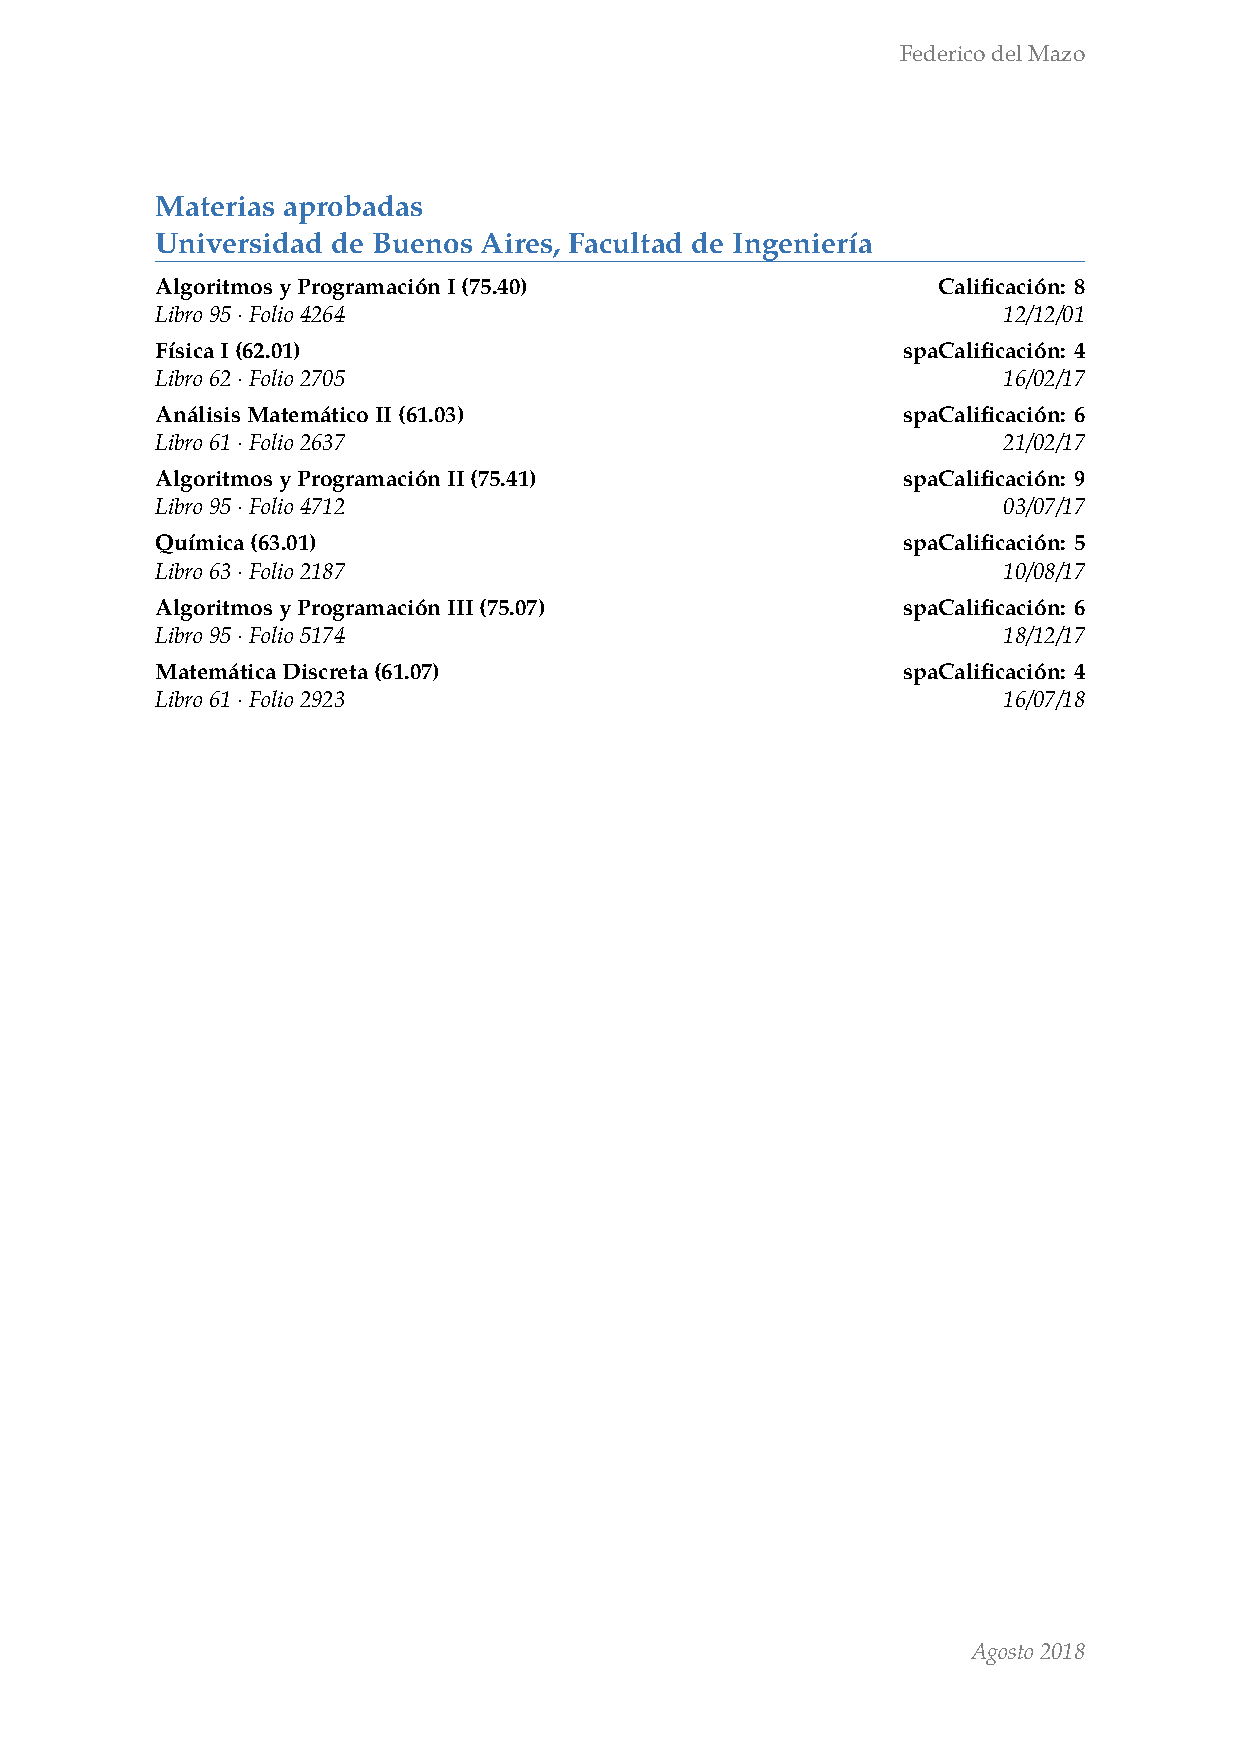
\includepdf[pages=-]{notas.pdf}}{}
\end{document}
"
\ifdefined\inenglish
  \entrue
\else
  \spatrue
\fi

% Márgenes
\usepackage[scale=0.75, top=2cm, bottom=2.5cm]{geometry}

% Lastpage para el footer (x paginas de y)
% Fontawesome para iconos en la cabecera
% Xpatch para cambiar el formato del titulo
% Framed (environment shaded*) y textpos (environment textblock*) para el 'boton' de cambio de lenguaje
% Setspace para el interlineado
\usepackage{lastpage,fontawesome,xpatch,framed,setspace}
\usepackage[absolute,overlay]{textpos}

% Interlineado 1.5
\onehalfspacing

% Sacar el 'subject' del PDF (era 'Resume of...') y cambiar el titulo (para que no sea "nombre - titulo")
\makeatletter
\AtEndPreamble{\hypersetup{pdfsubject={},pdftitle={\@firstname~\@familyname}}}
\makeatother

% Comando de mes en español, para el footer
\newcommand{\MONTH}{%
  \ifcase\the\month
  \or \spa{Enero}\en{January}
  \or \spa{Febrero}\en{February}
  \or \spa{Marzo}\en{March}
  \or \spa{Abril}\en{April}
  \or \spa{Mayo}\en{May}
  \or \spa{Junio}\en{June}
  \or \spa{Julio}\en{July}
  \or \spa{Agosto}\en{August}
  \or \spa{Septiembre}\en{September}
  \or \spa{Octubre}\en{October}
  \or \spa{Noviembre}\en{November}
  \or \spa{Diciembre}\en{December}
  \fi
}

% Cambiar formato de título (en vez de 'Autor | Curriculum' ahora es 'Autor \n Curriculum')
\makeatletter
\xpatchcmd{\makehead}{\titlestyle{~|~\@title}}{\par\vskip1ex\titlestyle{\@title}}{}{}
\makeatother

% Achicar el subtítulo ('Curriculum Vitae')
\renewcommand*{\titlefont}{\fontsize{21}{25}\mdseries\upshape}

% Header y Footer
\makeatletter
\fancyhead[R]{\color{gray}\@firstname{}~\@familyname{}}
\ifnum\value{page} > 1
  \fancyfoot[R]{\color{gray}\textit{\MONTH \the\year \\ \thepage/\pageref*{LastPage}}}
\else
  \fancyfoot[R]{\color{gray}\textit{\MONTH \the\year}}
\fi
\makeatother

% Solo footer para la primera pagina
\fancypagestyle{onlyfooter}{
\fancyhf{}
\ifnum\value{page} > 1
  \fancyfoot[R]{\color{gray}\textit{\MONTH \the\year \\ \thepage/\pageref*{LastPage}}}
\else
  \fancyfoot[R]{\color{gray}\textit{\MONTH \the\year}}
\fi
}

% Cambiar color de boton de lenguajes. Mientras mas cerca de 1, mas claro.
\definecolor{shadecolor}{gray}{0.9}
